\documentclass[class={myRUCProject}, crop=false]{standalone}

\usepackage[subpreambles = true]{standalone}
\usepackage{myTikz}




\IfStandalone{
    \usepackage[disable]{todonotes}
    \import{../../}{customCommands}
    \import{../../}{INP-00-glossary}
    }{}

\begin{document}

%A cell is the basic unit of life, a collection of matter with the ability to perform all the processes necessary for life, including reproducing itself. A multi-cellular organism, like humans, is composed of a number of independent cells maintained by complex interactions. How could anyone ever expect these meaty lumps we call `\textit{\glspl{gls:person}}' to coordinate properly without an equally complex system for the transfer of information? \Glspl{gls:neuron} are information highways made manifest in multi-cellular organisms. There exist many distinct types of \glspl{gls:neuron}, however, the underlying mechanisms of function stay the same.

%Of whether they be common skin cells or neuronal, those relevant to this project include the specialized form that neuronal cells have, as well as the ion channels and pumps that allow for the propagation of \gls{ap}, discussed in \Cref{sec:ap}.

\section{Specialized Neuronal Structures}

While sharing resemblances with other types of cells, neurons possess distinct properties that differentiate them from the rest and grant them special features that allow them to perform their selected tasks. One of its unique characteristics is the neuronal structure \cite{lovinger2008communication}.

\begin{figure}[H]
    \centering
    \import{../../Pictures/Anakin}{Neuron.tex}
    \caption{A simplified representation of a \gls{gls:neuron}[al] cell, with labels for each of the important features. (1) the \gls{gls:soma} of the cell; (2) a \gls{gls:dendrite}; (3) the \gls{gls:axon}; (4) the \gls{gls:ax-hill}; (5) the \gls{gls:ax-terminal}.}\label{fig:Neuron}
\end{figure}

There exist a number of important features that are foundational to the specialized functions found in the \glspl{gls:neuron};

\begin{enumerate}
    \item \glslink{gls:dendrite}{\textbf{The dendrites}} of a \gls{gls:neuron} are extensions of the \gls{gls:membrane} branching from the main body of the neuron - the soma. This overall shape and structure are metaphorically referred to as a `\textit{\gls{gls:denTree}}'.\footnotemark~This is where the majority of \gls{gls:neuron} inputs are received, and carried by the `dendritic spine' down to the \gls{gls:soma}~\cite{Hammond2015ch3,Hammond2015ch4}. \footnotetext{Greek root word `\textit{dendron}' meaning tree, translates to `tree tree'.}
    \item \glslink{gls:soma}{\textbf{The soma}} is the main body of the \gls{gls:neuron}. It is the space in which the nucleus resides, and by extension where protein production occurs. The nucleus can range from \qtyrange{3}{18}{\um} in diameter \cite{Hammond2015ch3,Hammond2015ch4}. This is exactly where the summation of all the electrical inputs received through the dendrites happens, which will determine whether or not a signal will be fired at the axon hill-lock. (An output signal in neurons is called an action potential.)
    \item \glslink{gls:axon}{\textbf{The axon}} is a finer tendril that can extend tens, if not tens of thousands of times, the diameter of the \gls{gls:soma} in length. The \gls{gls:axon} primarily carries nerve signals away from the \gls{gls:soma} and carries some types of information back to it. Most \glspl{gls:neuron} have only one \gls{gls:axon}, but this \gls{gls:axon} will be able to undergo significant branching, enabling communication with many target cells \cite{Hammond2015ch3,Hammond2015ch4}. 
    \item \glslink{gls:ax-hill}{\textbf{The axon hill-lock}} is the part of the \gls{gls:axon} where it emerges from the \gls{gls:soma}. The region contains the greatest density of voltage-dependent sodium channels, which makes it the most excitable part of the \gls{gls:neuron}and subsequently the site of impulse initiation~\cite{Hammond2015ch3,Hammond2015ch4}. 
    \item \glslink{gls:ax-terminal}{\textbf{The axon terminal}} is found at the terminus of the \gls{gls:axon} and is the region which establishes connections to other neurons  \cite{Hammond2015ch3,Hammond2015ch4}. 
    \item \glslink{gls:myelin}{\textbf{The myelin sheathe}} is a lipid and protein comprised substance excreted from Schwann cells\alextodo{} that `sheathes' the \gls{gls:axon}, creating additional insulation for \gls{gls:capa}~\cite{Hammond2015ch4}.
\end{enumerate}

% Interneuronal communication}

%The nineteenth-century observations by Camillo Golgi and Ramon Cajal on a structure of neurons led to the formulation of two contrasting propositions concerning how neurons communicate with each other. The first working theory was that neurons create netlike structures, resembling the cell arrangement of a heart muscle, thereby establishing a direct transmission of signals through the openings in the neuronal membrane. The second conjecture contended that neurons exist as single cells separated by membranes. The transmission in this case should occur via specific points allowing for chemical signalling between adjacent cells. Although initially in stark opposition, either one has been accurate, and so both means of communication are recognized to contribute to the signal propagation in the brain of mammals \cite{SHOYKHET2011783}.

As was initially suggested by Ramon y Cajal, the information flows from one neuron to the other at points where the axon terminal of one neuron connects to the dendrites of another. These points of contact between neurons that specialize in signal transmission are termed synapses. Synaptic neuronal communication constitutes a mechanism for rapid impulse transmission \cite{Hammond2015ch6}. 

Cells in the nervous system interact through a mixture of electrical signals (such as electrically charged ions) and chemical signals (e.g., neurotransmitters) \cite{lovinger2008communication} in order to communicate with other cells and and systems \cite{SHOYKHET2011783}. As such, there exist a few types of synapses which include electrical, chemical and mixed type synapses \cite{Hammond2015ch6, SZCZUPAK201699}. 
%Note that synaptic neural communication constitutes a mechanism for rapid impulse transmission. The information is predominately modulated by two classes of synaptic links \cite{SZCZUPAK201699}. Key distinctions between these transmission techniques include the speed of the signal, its accuracy, and that electrical synapses may possibly allow communication in the opposite direction \cite{SZCZUPAK201699}. Yet there are alternative modes of neural transport, thus the communication can occur through mechanisms beyond synaptical scope. Such variants contribute to the overall complexity and adaptability of the nervous system. [??add] 

%All cells in the nervous system interact through the mixture of electrical and chemical signals \cite{lovinger2008communication}, employing a variety of communication strategies, to reach other organs, muscles, and systems \cite{SHOYKHET2011783}. 
%The information is predominately passed via synaptic links, but the communication can also occur through mechanisms beyond the synaptical scope. 
%There are alternative modes of neural transport, such as gap junctions (electrical synapses) or volume transmissions [??]. These variants contribute to the overall complexity and adaptability of the nervous system [??]. 

%\subsubsection{Chemical synapses}
Chemical transmission is made feasible by small distances between the membranes of the connected cells (usually from 20 to 50 nanometers). The space that separates such neurons is called a synaptic cleft. The signal transmission involves a utilization of substances, called neurotransmitters, acting as chemical messengers. They are released by a presynaptic cell (i.e., neuron) into the synaptical cleft. Neurotransmitters bind to specific proteins on the dendritic membrane, known as receptors, which in turn modulate the opening of specific ion channels (gateways of ion flow), which ultimately regulates signal transmission, as will be elaborated further in the paper. In addition to neurotransmitters, there are also other substances, i.e., neuromodulators, hormones, that may not necessarily be released into the synaptic junction but contribute to chemical signal propagation \footnote{This statement is broad enough to include a range of neural cells (etc. glial or endocrine cells) beyond just neurons.} \cite{Hyman2005}.

%\subsubsection*{Electrical Synapses}

In the case of electrical synapses (or gap junctions), the membranes of the connected neurons are in close contact with each other. Here the flow of ions is not regulated by neurotransmitters, ions flow from one cell to the other directly.
%Neurons are in reality mutually isolated due to the presence of external membranes, preventing the direct contact, that would allow them to immediately exchange electrical and chemical signals. Contrary to this case is found within electrical synapses. The protein-based pores, named connexins \cite{sohl2005expression}, facilitates an immediate movement of ions through the closely bounded gap junctions, each of them comprising multiple connexin \footnote{Connexins are not ion channels themselves. They are fundamental compartments of gap junctions, specialized channels facilitating intercellular communication.} channels \cite{SZCZUPAK201699}. They link cytoplasms of two neighbouring neurons, enabling diffusion of ions and small group of atoms (like glucose) among cells \cite{SZCZUPAK201699}, and therefore bypassing the necessity for chemical transmitters \cite{kandel2000principles}. This way, neurons can exchange information regarding their metabolic processes (energy management), and excitability (network dynamics) \cite{SZCZUPAK201699}. Furthermore, myelin structure (sheath) that is generated by glial cells (Schwann cells in PNS, oligodendrocytes \footnote{The predominant subtype of glial cells forming the majority of the human central nervous system \cite{wei2019histology}.} in CNS) connects through gap junctions, producing additional structural support and permitting an immediate diffusion of nutrients in the direction of an axon\cite{SHOYKHET2011783}. Intercellular signal propagation via electrical synapses significantly influences the maturation of the nervous system. It persists, albeit to a lesser extent, in the adult nervous systems of both invertebrates and vertebrates \cite{SZCZUPAK201699} but it is relatively infrequent within the mammalian central nervous system, compared to the chemical transmission \cite{lovinger2008communication, sohl2005expression}. 

Additionally, a synaptic connection may be a combination of an electrical and a chemical synapse. Between neurons in mammals, mixed synapses are more common than the electrical ones \cite{Hammond2015ch6}
\begin{figure}
    \centering
    \begin{subfigure}[t]{0.3\textwidth}
        \centering
        \caption{}
        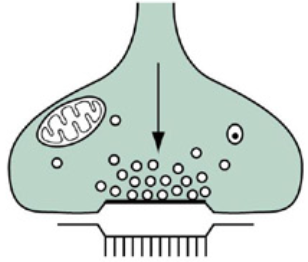
\includegraphics[height=3.7cm]{Pictures/Anakin/chem.syn.png}
    \end{subfigure}
    \begin{subfigure}[t]{0.3\textwidth}
        \centering
        \caption{}
        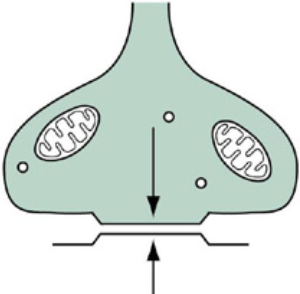
\includegraphics[height=4cm]{Pictures/Anakin/el.syn.png}
    \end{subfigure}
    \begin{subfigure}[t]{0.3\textwidth}
        \centering
        \caption{}
        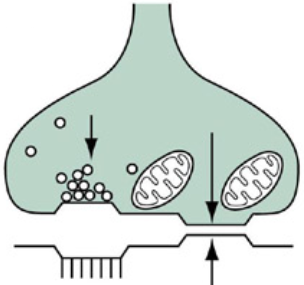
\includegraphics[height=4cm]{Pictures/Anakin/mix.syn.png}
    \end{subfigure}
    \caption{Types of synapses. (a) Chemical synapse; (b) electrical synapse (gap junction); (c) mixed synapse. From \cite{Hammond2015ch6}}\label{fig:synapses} 
\end{figure}

\section{The Resting Membrane Potential} 
A fundamental component of cells is the \gls{gls:membrane}, composed of what is known as a \gls{gls:bilipid}.{}\footnote{Latin root word `bi' meaning two, translates to `lipid two-layer'} 
A \gls{gls:bilipid} creates a strong electrical insulation, which confers\anakintodo{We need to remember to elaborate} it the property of `\gls{gls:capa}'~\cite{Hammond2015ch3,Hammond2015ch4}.{}\footnote{The capability of an object to store electrical charge.}
In a \gls{gls:neuron}, the overall charge in the \gls{gls:incell} space is more negative relative to the \gls{gls:excell} space. This difference in charge at rest is known as the resting \gls{gls:mPote}, and it is essential for the \gls{gls:neuron}['s] ability to transmit electrical signals \cite{Hammond2015ch3,Hammond2015ch4}. 

By convention, membrane potential - \(\br{\unit{\V\membrane}}\) is the difference between the electric potential of the internal and external faces of the membrane \(\br{\unit{\V\membrane}=\unit{\V\incell}-\unit{\V\excell}}\). In the absence of ongoing electrical activity, this negative potential is termed the resting membrane potential \(\br{\unit{\V\rest}}\). The usual resting \gls{gls:mPote} is found to be around \glslink{gls:volt}{\qty{-70}{millivolts\br{\milli\volt}}} in \glspl{gls:neuron}, however, it varies depending on the cell type and conditions~\cite{Hammond2015ch3,Hammond2015ch4}. When the membrane potential is less negative than \(V_{rest}\), the membrane is considered to be depolarized. In contrast, when the membrane potential is more negative than \(V_{rest}\), the membrane is said to be \gls{gls:hypol} \cite{Hammond2015ch3}. 

The \glspl{gls:ion} primarily involved in the \gls{gls:mPote} include \gls{Na}, \gls{K}, \gls{Cl}, and, to a limited degree, \gls{Ca}. 
In the \gls{gls:excell} space the concentrations of \gls{Na} and \gls{Cl} are kept much higher than in the cytoplasm\kennitodo{perhaps explain?} of the \gls{gls:incell} space, whereas \gls{K} is found in much higher concentrations in the cytoplasm compared to the \gls{gls:excell} space. 
During rest, their concentration \glspl{gls:grad} are actively regulated and maintained at constant values by `\glspl{gls:ionPump}' chemically transporting \glspl{gls:ion} across the \gls{gls:membrane}~\cite{Hammond2015ch3,Hammond2015ch4}. 
However, the main contributors to the negative potential of the intracellular side of the \gls{gls:membrane} are the anions of the intracellular fluid, which are organic molecules such as negatively charged amino acids, proteins, nucleic acids, phosphates, etc., which have a large molecular weight and cannot cross the lipid membrane and thus do not participate directly in electrical signaling in neurons~\cite{Hammond2015ch3}. 


\subsection{Ion channels}
%An important structure embedded in the \gls{gls:bilipid} includes `\glspl{gls:ionChan}' which permit electrically charged \glspl{gls:ion} to diffuse across the \gls{gls:membrane} \gls{gls:grad}. \Glspl{gls:ionChan} are only permeable to a specific \gls{gls:ion}~\cite{Hammond2015ch4}. Some \glspl{gls:ionChan} are \gls{gls:vgate}[d], meaning that they can be switched between open and closed states by altering the voltage across the \gls{gls:membrane}. 
%Others are `\gls{gls:lig} gated', meaning that they can be switched between an open and a closed state by interacting with \glspl{gls:lig} that travel through the \gls{gls:excell} fluid. 

An important structure embedded in the \gls{gls:bilipid} includes `\glspl{gls:ionChan}', specialized proteins which permit electrically charged \glspl{gls:ion} to diffuse across the \gls{gls:membrane} \gls{gls:grad}, producing electric current (this will be elaborated in the following sections). Thus, neurons are cells that manifest excitability as their characteristic feature. 

Ion channels are not confined to synapses or dendrites, but are distributed across the whole outer membrane. However, ion channels highly selective and are only permeable to a specific \gls{gls:ion}~\cite{Hammond2015ch4}. Membranes may  contain various types of these channels,  like sodium (\gls{Na}), potassium (\gls{K}), calcium (\gls{Ca}), and chlorine (\gls{Cl}), which are all essential for neuron excitability and  (electrical) signal propagation.


Some \glspl{gls:ionChan} are \gls{gls:vgate}[d], meaning that they can be switched between open and closed states in response to changes in the voltage across the \gls{gls:membrane}. 
Others are `\gls{gls:lig} gated', meaning that they  open upon binding of certain molecules (\gls{gls:lig}[s]) like neurotransmitters, released into the synaptic cleft by the presynaptic neuron. The coupling of neurotransmitters to receptors on a postsynaptic dendritic membrane initiates a reaction in a postsynaptic cell, which leads to either depolarization (excitation) or hyperpolarization (inhibition). The outcome is contingent on the class of the neurotransmitter, the specific protein – receptor interaction, and the neuronal circuitry.

%The overall concept of ion channels is unique to the field of biology and neuroscience. The terminology may vary based on the field, meaning that in the context of physics or materials science one may write about the electron or proton channels instead, when discussing the passage of charged particles.

%Ion channels are highly selective, they permit the transition of only a certain class of charged particles – as the name suggests, ions. 
%they are implicitly designed to accommodate the flow of specific ions, dependent upon the channel’s characteristics. 
%Membranes may  contain various types of these channels,  like sodium (Na+), potassium (K+), calcium (Ca2+), and chloride (Cl-), which are essential for the (electrical) signal propagation including action potentials, excitability of a neuron, and some other cell functions.

%The movement of ions and the channel selectivity is often determined by the size and charge of the specific atom they transport. 
%But one can also say this the other way round. The structure of an ion channel comprises a pore through which ions traverse and so that the dimensions and shape of the pore dictates exactly which ion is permitted to go through, excluding every other. 
% For other charged particles, such as electrons or protons, even though they are notably smaller and distinctly charged, neither one of them is commonly transported through ion channels, since these types of atoms are beyond the scope of biological systems. 

\begin{figure}[H]
  \centering
  \import{../../Pictures/Anakin}{Channels.tex}
  \caption{ $\langle \text{temp, will become channels/pumps} \rangle$ }\label{fig:Channels}
\end{figure}\todo{Make name}

\subsection{Ions Diffuse Downstream of Their Electrochemical Gradient}\label{sec:diffuseIon}

The direction of the diffusion of \glspl{gls:ion} through an open channel depends on both the concentration \gls{gls:grad} of the \gls{gls:ion} and the \gls{gls:mPote}. The resulting combination of these two forces is called the electrochemical \gls{gls:grad}.

For instance, when the \gls{gls:mPote} is null \(\br{\unit{\V\membrane}=\qty{0}{\mV}}\), there is no difference of \gls{gls:Pote} between the two faces of the \gls{gls:membrane}, so the concentration \gls{gls:grad} will be the only factor determining the direction of diffusion for specific \glspl{gls:ion}. 
Since the concentrations of \gls{Na}, \gls{Ca} and \gls{Cl} in the \gls{gls:excell} fluid are higher, on average, than in the \gls{gls:incell} medium, these \glspl{gls:ion} will diffuse passively towards the \gls{gls:incell} space,\footnote{via \gls{Na}, \gls{Ca} or \gls{Cl} permeable ion channels}~as a result of their concentration \gls{gls:grad}. 
In contrast, since \gls{K} is a lot more abundant in the intracellular \gls{gls:media}, it will move from the \gls{gls:incell} \gls{gls:media} to the \gls{gls:excell} one when \gls{K} permeable channels are open. 

If we suppose that there is the same concentration of each \gls{gls:ion} in the \gls{gls:excell} and \gls{gls:incell} \glspl{gls:media}, i.e there is no concentration \gls{gls:grad} for any \glspl{gls:ion}, \glspl{gls:ion} will diffuse according to \gls{gls:mPote} only: positive ions (cations) will move towards negative potential, negative ions (anions) will move towards postive \gls{gls:Pote}. At a \gls{gls:mPote} \(\unit{\V\membrane}=\qty{-30}{\mV}\), positively charged \glspl{gls:ion}, the \glspl{gls:cation} \gls{Na}, \gls{Ca} and \gls{K}, will move from the \gls{gls:excell} \gls{gls:media} to the \gls{gls:incell} one according to \gls{gls:mPote}. In contrast, \glspl{gls:anion} (\gls{Cl}) will move from the \gls{gls:incell} \gls{gls:media} to the \gls{gls:excell} one. 


In physiological conditions, the concentration \gls{gls:grad} is maintained constant for each \gls{gls:ion}, so the direction and amplitude of diffusion mainly varies with \gls{gls:mPote}. The resultant of these two potentials, concentration and \gls{gls:Pote} \glspl{gls:grad}, is the electrochemical \gls{gls:grad}. To know how to express the electrochemical \gls{gls:grad}, the \gls{gls:ePote} must first be explained.
 
\subsection{Equilibrium Potential}
\begingroup
\allowdisplaybreaks
All systems yearn for their \gls{gls:equil}, the fabled \textit{steady state}. This divine relation of the components in a system, one achieved, the system no longer needs to evolve, it has been perfected by \gls{gls:entropy}.
The value of the \gls{gls:mPote} is constantly fluctuating depending on the relative distribution of charged particles that cross the \gls{gls:membrane}.

When the \glspl{gls:grad} are balanced at net zero, it is referred to as the \gls{gls:ion}[ic] \textbf{\gls{gls:ePote}[s]} \br{\equi\ion}, alternatively, as the `\gls{gls:rPote}' of the \gls{gls:ion} \(\equi\reverse\). 
The \(\equi\ion\) of the given \glspl{gls:ion} can be calculated using the \emph{Nernst equation} for equilibrium potential of an ion species:
\begin{subequations}\label{eq:nernst}
\begin{equation}
  \equi\ion = \unit{\V_{\ionconc\incell}} - \unit{\V_{\ionconc\excell}} = \br{\frac{\clm{R}\, \cdot \,\clm{T}}{z\, \cdot \, \clm{F}}} \, \ln \br{\frac{\ionconc\excell }{ \ionconc\incell} } \tag{\ref*{eq:nernst}}
\end{equation}
Where \(\clm{R}\) is the ideal gas constant \br{\qty{8.314}{\cubic\meter\pascal\per\kelvin\per\mol}}; \(\clm{T}\) is the temperature in \gls{gls:kelvin} \(\br{ x\,\unit{\glssymbol{gls:celsius}} \cong {273.15} + x\,\unit{\kelvin}}\); \(\clm{F}\) is the Faraday constant \br{\qty{96500}{\coulomb\per\mole}}; \(z\) is the valence of the \gls{gls:ion}; and \(\ionconc\) is the concentration of the given \gls{gls:ion} in the \gls{gls:excell} \( \br{ \clm{E} } \) or \gls{gls:incell} \( \br{\clm{I}}\) \gls{gls:media}. 

\end{subequations}

\begin{subequations}\label{eq:mVions}
With minor adjustments\footnote{Left as an exercise for the reader} to \cref{eq:nernst}, one is able to derive;
\begin{equation}
  \equi\ion = \cfrac{\clm{T}\unit{\per\K}}{ z } \, \cdot \, \ln \br{ \frac{ {\ionconc\excell} }{ {\ionconc\incell}} } \cdot \num{11.612515042}^{-1} \ \unit{\milli\volt} \tag{\ref*{eq:mVions}}
\end{equation}

Plugging the relative concentrations, measured in millimoles \br{\unit{\milli\mol}}, of each \gls{gls:ion} into \cref{eq:mVions}, as well as choosing an arbitrary temperature, such as human body temperature \(\approx\) \qty{37}{\degreeCelsius} \(\br{\sbr{\num{37} + \num{273.15}}\unit{\glssymbol{gls:kelvin}}}\),
using the relevant \(\ionconc\),
the \glspl{gls:ePote} follow:\par
\noindent
\scalebox{0.90}{
\begin{minipage}[c]{.525\textwidth}
  \begin{align}
    {\equi\sodium} &= \num{310.15}\ \ln \br{ \frac{142}{15} }\cdot \num{11.612515042}^{-1} &=& \qty{60.034194963084595}{\mV} \label{eq:Na}\\
    {\equi\potassium} &= \num{310.15}\ \ln \br{ \frac{4}{150} }\cdot \num{11.612515042}^{-1} &=& \qty{-96.79981780837547}{\mV} \label{eq:K}
    \end{align}
\end{minipage}}
\hfill
\scalebox{0.90}{
\begin{minipage}[c]{.525\textwidth}
  \begin{align}
    {\equi\chlorine} &= \num{-310.15}\ \ln \br{ \frac{120}{\num{5}} }\cdot \num{11.612515042}^{-1} &=& \qty{-84.88026856520263}{\mV} \label{eq:Cl}\\
    {\equi\calcium}  &= \frac{310.15}{2}\ \ln \br{ \frac{1}{\num{e-4}} }\cdot \num{11.612515042}^{-1} &=& \qty{122.99605451690456}{\mV} \label{eq:Ca}
  \end{align}
\end{minipage}}
From here, we now know where limitations in the range \(\unit{\V\reverse}\) might exist.

\end{subequations}

\endgroup

\subsection{Ionic currents}
The passive diffusion of \glspl{gls:ion} through an open channel implies a movement of charge through some resistance. Current comes from the movement of charge.
When focusing on a single channel, the current is called `single-channel current' or `unitary current', \(\br{\ucur\ion}\). The amplitude of \(\ucur\ion\) is expressed in ampere \(\br{\unit{\ampere}}\) which are coulombs per seconds \(\br{\unit{\coulomb\per\second}}\). 

In general, currents are expressed following Ohm's law: \(\rmm{U}=\rmm{Z}\curr\), where \(\curr\) is the current through a resistance \(\rmm{Z}\) and \(\rmm{U}\) is the difference of \gls{gls:Pote} between the two ends of the resistance. 
For currents created by \gls{gls:ion}[ic] charge (and not by electrons as in copper wires), \(\curr\) is labeled \(\curr\ion\), the current that passes through the resistance of the channel pore which has a resistance \(\rmm{R}\) \(\br{\res\ion}\). 

But what is \(\rmm{U}\) in biological systems? 

\unit{U} is the electrical potential, directing the \glspl{gls:ion} along a particular axis; it is the electrochemical \gls{gls:grad} for the considered \gls{gls:ion} and is also called the driving potential: \(\rmm{U}=(\unit{\V} - \equi\ion)\). According to ohm's law, the current \(\curr\ion\) through a single channel is derived from 
\begin{equation}
  \unit{\V} - \equi\ion = r\ion \cdot \curr\ion
\end{equation}
So:
\begin{equation}\label{eq:cur2con}
  \curr\ion= \frac{1}{r\ion\br{\unit{\V} - \equi\ion}} = \ucon\ion(\unit{\V\membrane} - \equi\ion)
\end{equation}

The measure of the \glspl{gls:ion} through a single channel, is called the unitary \gls{gls:contan} \(\br{\ucon\ion}\) which is the real part of \gls{gls:admit}. 
The reciprocal of resistance; it is called the \textit{\gls{gls:admit}}.
While resistance is expressed in \gls{gls:ohm} \(\br{\unit{\ohm}}\), \gls{gls:admit} is expressed in siemens \(\br{\unit{\siemens}}\).\footnote{\Gls{gls:admit} can also be expressed in `mho' which is inverse ohm, \(\unit{\ohm}^{-1} = \unit{\mho}\)}~
By convention \(\curr\ion\) is negative when it represents an inward \gls{gls:flux} of positive charges (\glspl{gls:cation}) and \(\curr\ion\) is positive when it represents an outward \gls{gls:flux} of positive charges. It is generally of the order of pico-ampere \(\br{\qty{1}{\pico\ampere}=\qty{e-12}{\ampere}}\). At physiological concentrations, \(\ucon\ion\) varies between \(\qtyrange{10}{150}{\pico\siemens}\) dependent on channel type~\cite{Hammond2015ch4}.

\(\curr\ion\) and \(\ucur\ion\) can be measured experimentally. 
The former is measured current from a patch of \gls{gls:membrane} where only one channel of a given type is present.
{}\(\curr\ion\) is current measured from a whole \gls{gls:membrane} where \(N\) channels of the same type are present. The techniques mainly used for measuring ionic currents in excitable cells are the current- and voltage- clamp techniques.

\subsubsection{Current clamp}\label{sec:Cclamp}

Current clamping is a technique for recording the membrane potential and how that potential changes by injecting current into a cell through the recording electrode.  
`Current clamp' implies that the current applied through the electrode is held at a constant value for the experiment, while the membrane potential is free to vary~\cite{Hammond2015ch4}. The amplifier records whatever voltage the cell generates on its own or as a result of stimulation. 
This technique is useful for studying how a cell responds when electric current enters a cell~\cite{Hammond2015ch4}.

\subsubsection{Voltage clamp technique}\label{sec:Vclamp}
 
In contrast to the current clamp technique, in voltage clamp mode the cell potential is `clamped' at a chosen value while recording changes in ionic currents~\cite{Hammond2015ch4}. 
This allows to measure how much \textit{ionic current} is flowing through the cell's membrane at any given voltage. 
This is important because, as will be elaborated in \Cref{sec:depol}, many of the ion channels in neuronal membrane are \gls{gls:vgate}[d] ion channels, which open only when the membrane voltage is within a certain range, and the voltage clamp technique allows for control of the variable determining the opening of those channels~\cite{Hammond2015ch4}. It controls the voltage across the membrane to a specific value so that the behavior of system in study is independent of it. Originally, this experiment was done on a squid axon since it was relatively larger than most and would allow for less intricate experimental setups.

\begin{figure}[H]
    \centering
    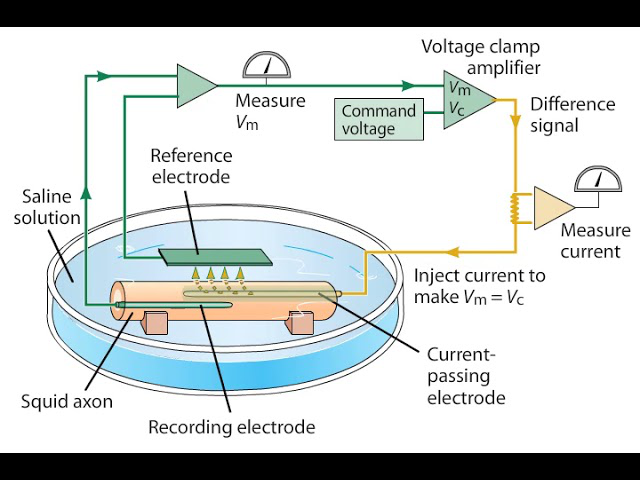
\includegraphics[trim=0 25 0 25,clip,width=0.55\textwidth]{Pictures/Ana/clamp.png}
    \caption{A visualization of the voltage. The \textbf{reference electrode} clamping method compares the voltage with the one inside in order to measure the voltage difference. The \textbf{command voltage} is the desirable voltage that is controlled by a diode that can drop the voltage according to the voltage difference. This will generate a current that will be injected back to the system. Such current will balance the voltage to the desirable one. The \textbf{measured current} is the current needed to keep the voltage the same as the command voltage. How the needs to vary in accordance to the ion channels will give insight into how the channels work(conductance for example) \cite{Purves}.}
\end{figure} 

% \textbf{ Reference electrode:} Compares the voltage with the one inside in order to measure the voltage difference.

% \textbf{Command voltage:} The desirable voltage that is controlled by a diode that can drop the voltage according to the voltage difference. This will generate a current that will be injected back to the system. Such current will balance the voltage to the desirable one.

% \textbf{ Measured current:} Current needed to keep the voltage the same as the command voltage. How the needs to vary in accordance to the ion channels will give insight into how the channels work(conductance for example).

A variation of voltage clamp technique is the patch clamp technique, which allows to isolate currents from patches of cell membrane or even individual ion channels~\cite{Hammond2015ch4}.

\section{The Action Potential}\label{sec:ap}

Recall that the resting potential is the value, the \gls{gls:mPote} maintains, as long as nothing perturbs the cell. The interior of the neuronal membrane at rest carries a negative charge relative to the exterior space \cite{wood1996neuroscience}. Membrane potentials typically fall within the range of \qtyrange{-40}{-90}{\mV} millivolts (Section 1.2) \cite{ramachandran2002encyclopedia}, and in human cells it is around {\qty{-70}{\milli\volt}} \cite{ Hammond2015ch4}. Action potentials (AP) cause a quick inversion of the above state so that the \gls{gls:incell} space ends up being positive and \gls{gls:excell} being negative, for some duration of time \cite{wood1996neuroscience}. This is done by injecting a positive electrical current into the cell \footnote{In neuronal somas and axons, these currents are most commonly propagated by \gls{Na} cations - positively charged ions (no relation to Felis Catus)}, leading to the depolarization of the cell membrane – a decrease in membrane potential \textit{negativity} \cite{ramachandran2002encyclopedia}. This positive inward flux of current causes adjacent regions of the cell to similarly 'depolarize', creating a chain reaction in the form of a 'wavelet' \cite{Hammond2015ch3}. The type of signal that we consider in this section predominantly occurs in axons. The other parts of the neuronal cell refrain from generating action potentials due to the limited presence of voltage-gated sodium channels in the membrane \cite{wood1996neuroscience}. Accordingly, the region known as the axon hillock is frequently referred to as the spike-initiation zone \cite{wood1996neuroscience}.

\subsubsection{Properties of Action Potential}
AP exhibits four general features, in the context of neuronal signal propagation \cite{kandel2000principles}. Biologists grappled with the enigma of these properties for nearly a century since the first measurement of the action potential. These features are unique to action potentials only, which stands out from typical biological processes \cite{kandel2000principles}. Research conducted by Hodgkin, Huxley, and Katz on the membrane properties of the giant squid axon, yielded some initial understanding \footnote{The pioneering and detailed account of the \gls{gls:ion}[ic] basis for \gls{gls:neuron}[al] excitation governing the action potential was first provided by Hodgkin and Huxley (1952) using the voltage clamp technique,  \cref{sec:Vclamp} \cite{HodHux1952,kandel2000principles}.}.

First of all, AP has a certain \textit{threshold}, or depolarization level, at which it is triggered. A threshold is a membrane potential at which the activation of a sufficient amount of voltage-gated sodium channels, shifts the ionic permeability of the membrane, favoring sodium over potassium \cite{wood1996neuroscience}. In a variety of nerve cells, the membrane exhibits a simple resistive behavior, allowing us to calculate the threshold potential \footnote{A very neat explanation provided by \cite{kandel2000principles}.}. Once the threshold voltage is achieved, usually at approximately {\qty{-50}{\milli\volt}}, an action potential is created \cite{kandel2000principles}. Which leads to the second property. 

The action potential follows an \textit{all-or-none} principle \cite{kandel2000principles}. It provides a maximal response when subjected to stimulation, so that the concept of a "strong" or "weak" spike is not applicable to action potentials [??]. Increasing the intensity of the stimulating current pulse does not increase the amplitude of the AP \cite{Hammond2015ch3}.

Thirdly, action potentials are transmitted without any reduction in signal strength, meaning they do not diminish as they propagate over the axon due to their consistent production in the axon hillock.
\footnote{Also due to the presence of insulating myelin sheaths, and the density of voltage-gated \gls{Na} channels remaining constant along the axon \cite{Hammond2015ch4}. Many types of \glspl{gls:neuron} emit \glspl{ap} constantly at rates of up to 10–100 per second. However, some types are much quieter, and may go for minutes or longer without emitting any \glspl{ap}.}
This property maintains a \textit{constant amplitude} even over long distances.

Lastly, after the signal is fired, there is a \textit{refractory phase} during which the neuronal capacity to generate a second action potential is temporarily restrained. Neuron shows decreased sensitivity to the new stimulus inhibiting instant response, i.e., re-excitation \cite{kandel2000principles}. That controls the frequency of action potential firing, placing constraints on the axon's ability to convey information \cite{kandel2000principles}. 

\subsubsection{Waveform}

Voltmeter records the electrical potential difference between the microelectrode's tip placed in the interior of the cell and the extracellular space. The resting membrane potential is, for the sake of argument, -70 mV. In most neurons, the entire process of neuronal spiking takes place in about a thousandth of a second, therefore action potentials are investigated using oscilloscopes, a specific category of voltmeters \cite{wood1996neuroscience}. \cref{fig:AP} illustrates an action potential, that is a plot of a membrane potential as a function of time. 


%\gls{ap} is all or none \cite{Hammond2015ch4}. 
\begin{figure}[H]
  \centering
  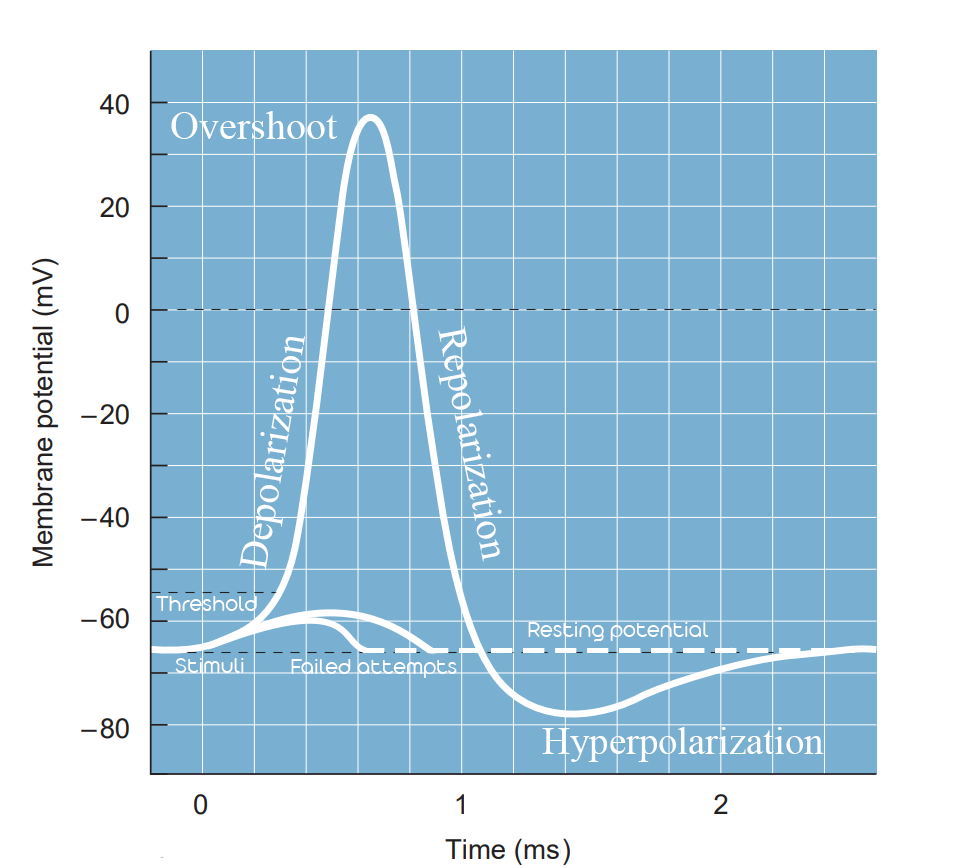
\includegraphics[width=0.6\linewidth]{Pictures/Svet/Untitled-1.png}
  \caption{The action potential spike, indicating the different phases, displayed by an oscilloscope \cite{wood1996neuroscience}.}\label{fig:AP}
\end{figure}


\begin{itemize}
\item Sodium ions experience a substantial driving force when the electrical potential inside the membrane is negative. They hurry inside the neuron, entering via the open (\gls{Na}) channels so that the membrane undergoes an instant depolarization \cite{wood1996neuroscience}. 

\item Up to the threshold level, only passive ohmic responses can be recorded [??]. However, when enough of this depolarization accumulates to bring the membrane \gls{gls:Pote} up to its threshold, around \qty{-55}{\mV} \cite{Hammond2015ch3}, AP is triggered. The curve on the graph abruptly ascends to the level well above 0 mV \cite{ramachandran2002encyclopedia}. This stage is called the \textbf{depolarization} or a rising phase. During this time span, the membrane experiences a significant depolarization, an electrochemical driving force makes potassium hurry to flow through open channels, making the membrane potential to revert to a negative state \cite{wood1996neuroscience}. This makes the voltage-gated potassium channels ultimately open, with some time delay. 

\item The membrane potential does not stop until it attains its maximum pinnacle, of approximately 40 mV \cite{wood1996neuroscience}. Once the membrane potential \unit{\V\membrane}\ reaches positive values, we are speaking about the stage of \textbf{overshooting}. This is because the membrane permeability strongly tilts in favor of sodium so that the potential approaches values akin to the \gls{Na} equilibrium potential \unit{\equi\sodium}\cite{wood1996neuroscience}, that is roughly \qty{60}{\mV}, (Section). The \gls{gls:flux} of \gls{Na} \glspl{gls:ion} triggers the opening of additional \gls{Na} channels in the axon segment, which cascades until all \gls{Na} channels in the segment have opened. This coincides with the \gls{gls:depol} phase reaching its peak \cite{Hammond2015ch4}.

\begin{figure}[b]

\centering
  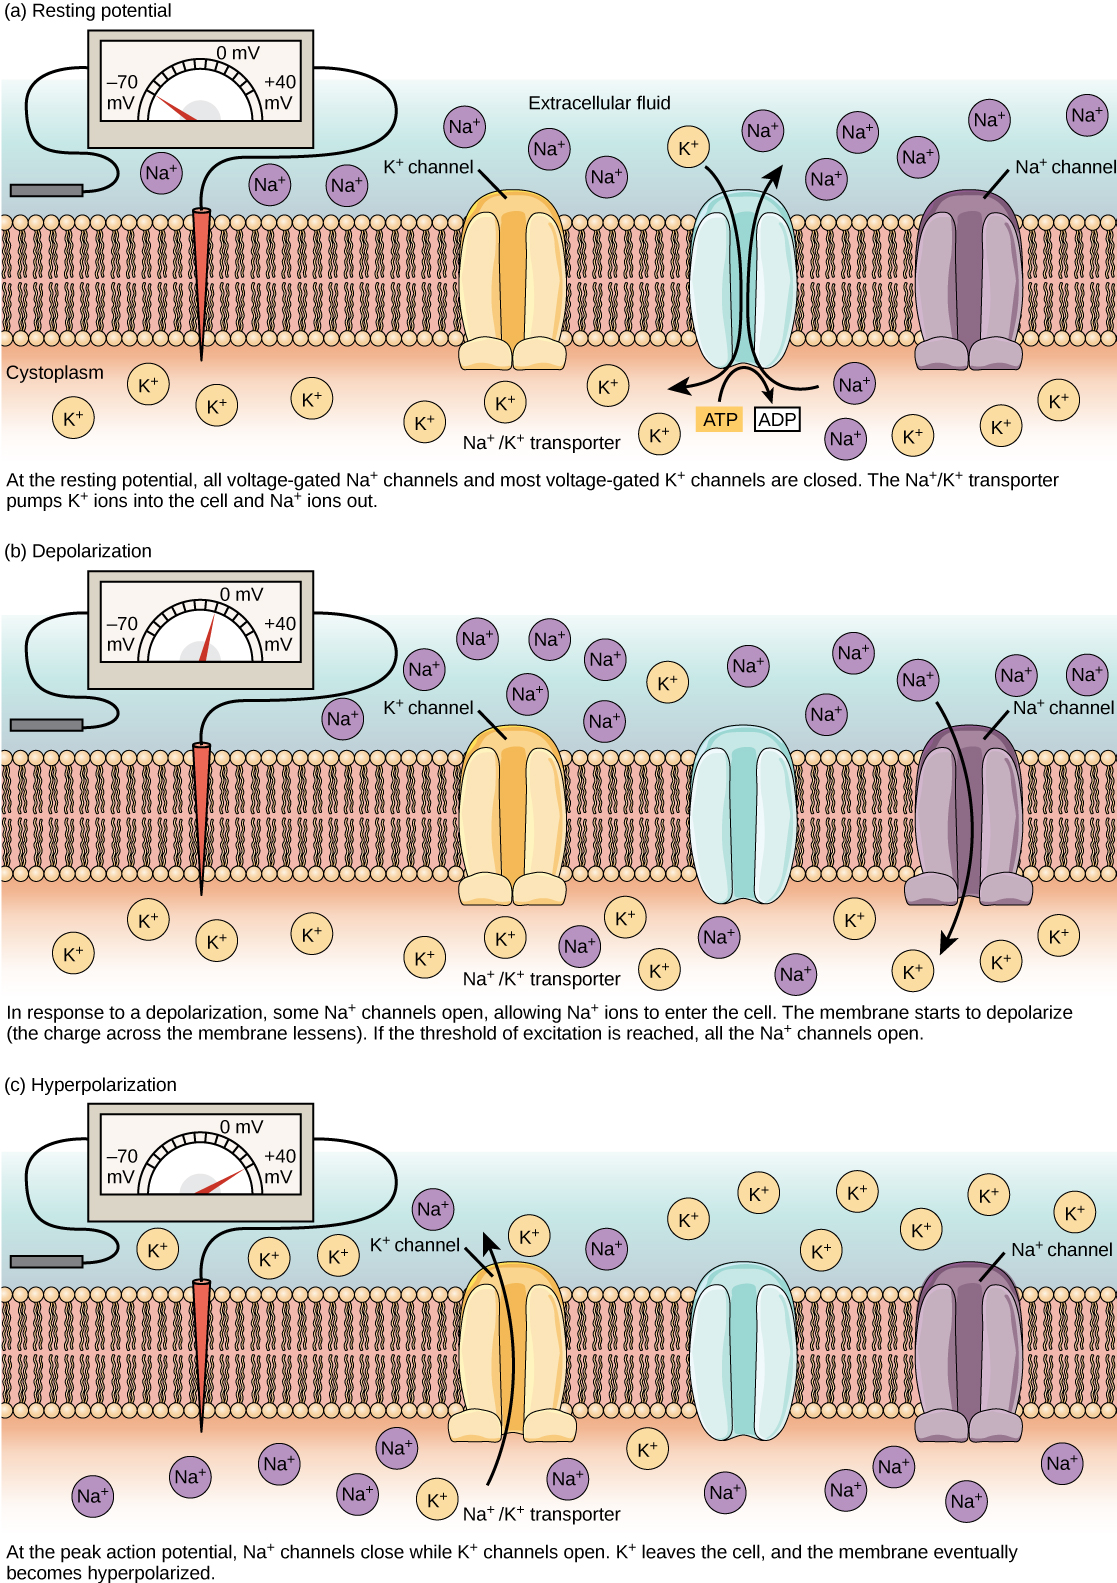
\includegraphics[width=0.6\linewidth]{Pictures/Svet/Ion_channel_activity_before_during_and_after_polarization.jpg}
  \caption{\textbf{Three main phases of the action potential spike.} The cellular membrane contains three classes of specific proteins, namely sodium voltage-gated channels (violet), potassium voltage-gated channels (orange), and potassium-sodium pumps (blue). Despite the omission of the topic of sodium-potassium pumps in the project, it is worth bearing in mind that sodium-potassium pumps are actively functioning in the background, sustaining the ionic concentration gradients and propelling sodium and potassium ions through their respective channels during spiking \cite{wood1996neuroscience}.
 }\label{fig:fasd}
\end{figure}


\item Within a span of \qtyrange{1}{5}{\ms}, the membrane potential equally abruptly descends back downwards \cite{ramachandran2002encyclopedia}, usually undershooting the resting value, where it remains for some period of time \cite{ramachandran2002encyclopedia}. What genuinely happens is that the membrane rapidly \textbf{re-polarizes}, which closes the voltage-gated sodium channels \cite{wood1996neuroscience}.

\item The fall lasts up to the point when the interior of the membrane becomes in fact, more negative than the resting potential. This final section of the declining phase is called the \textbf{hyper-polarization} \cite{wood1996neuroscience}. Its restoration can sometimes incidentally trigger an action potential on its own (rebound spiking) \cite{ramachandran2002encyclopedia}. Remember, that the voltage-gated potassium channels are still active, making the permeability of the membrane lean toward the potassium. As a result, the membrane potential approaches values closer to \gls{K} equilibrium potential \unit{\equi\potassium}\, (Section), due to the minimal sodium movement, undershooting the resting potential \cite{wood1996neuroscience}. The membrane stays hyper-polarized until the voltage-gated potassium channels inactivate themselves.
\end{itemize}



%\subsubsection{Depolarization of the membrane potential}\label{sec:depol}

%The threshold for initiation of \gls{Na}[-dependent] action \gls{gls:Pote} is due to \gls{gls:vgate}[d] \gls{Na} channels only opening in response to a \gls{gls:depol} of \qtyrange{-50}{-40}{\mV}, hence the classification `\gls{gls:vgate}[d]' \cite{Hammond2015ch4}. 

%In response to \gls{gls:depol} passing the \gls{gls:tPote}, closed \gls{Na} channels of the axon segment\anakintodo{Need to elaborate that model only represents discrete segments of the axon} begin to open. The \gls{gls:flux} of \gls{Na} \glspl{gls:ion} through the open \gls{Na} channels depolarize the \gls{gls:membrane} more, triggering the opening of additional \gls{Na} channels. 
%Consequentially, the \gls{gls:flux} of \gls{Na} \glspl{gls:ion} increases, causing further \gls{gls:depol} of the \gls{gls:membrane}, cascading until all \gls{Na} channels in the segment have opened. 
%This coincides with the \gls{gls:depol} phase reaching its peak \cite{Hammond2015ch4}. 

%{}\gls{Na} channels are opened by \gls{gls:depol} and once opened, they reinforce the \gls{gls:membrane} \gls{gls:depol} and therefore their own activation: a self-maintained process,\footnotemark~which is why the \gls{Na}[-dependent] \gls{ap} is all or none.\footnotetext{Also commonly referred to as a `positive feedback cycle'.}
%Once initiated, the \gls{ap} propagates along an axon without decaying in amplitude, at rates ranging between \qtyrange{1}{100}{\meter\per\s}. 
%This propagation proceeds without \gls{gls:attenuation} due to the density of \gls{gls:vgate}[d] \gls{Na} channels remains constant along the axon; as well due to the presence of insulating \glspl{gls:myelin}. 
%Once the channels become inactive, they may not reopen, ensuring that \gls{ap} only propagates forward. 

%The time during which the \gls{Na} channel stays open is the mean open time, denoted \(\tau_o\) \cite{Hammond2015ch4}.\footnote{The letter  `o', not the number `0'}

\subsubsection{Propagation}

The way the action potential travels along the axon is much like a flame moving along a fuse \cite{wood1996neuroscience}. Recall, that when a section of axonal membrane experiences sufficient depolarization to surpass the threshold it triggers the opening of voltage-gated sodium channels, creating an action potential. The flow of the positive charge extends through the axon causing a further depolarization of neighboring segments if they too, reach the threshold value. In this manner, the action potential travels down the axon until it reaches the terminal, commencing an interneuronal communication \cite{wood1996neuroscience}. The signal travels exclusively in one direction, because of the refractory period resulting from closing sodium channels, guaranteeing the unidirectional propagation of the action potential \cite{Hammond2015ch4}. Similar to the fuse scenario, the signal might initiate from both tails of the axon upon depolarization, allowing for bidirectional transmission \cite{wood1996neuroscience}.

\begin{figure}[H]
  \centering
  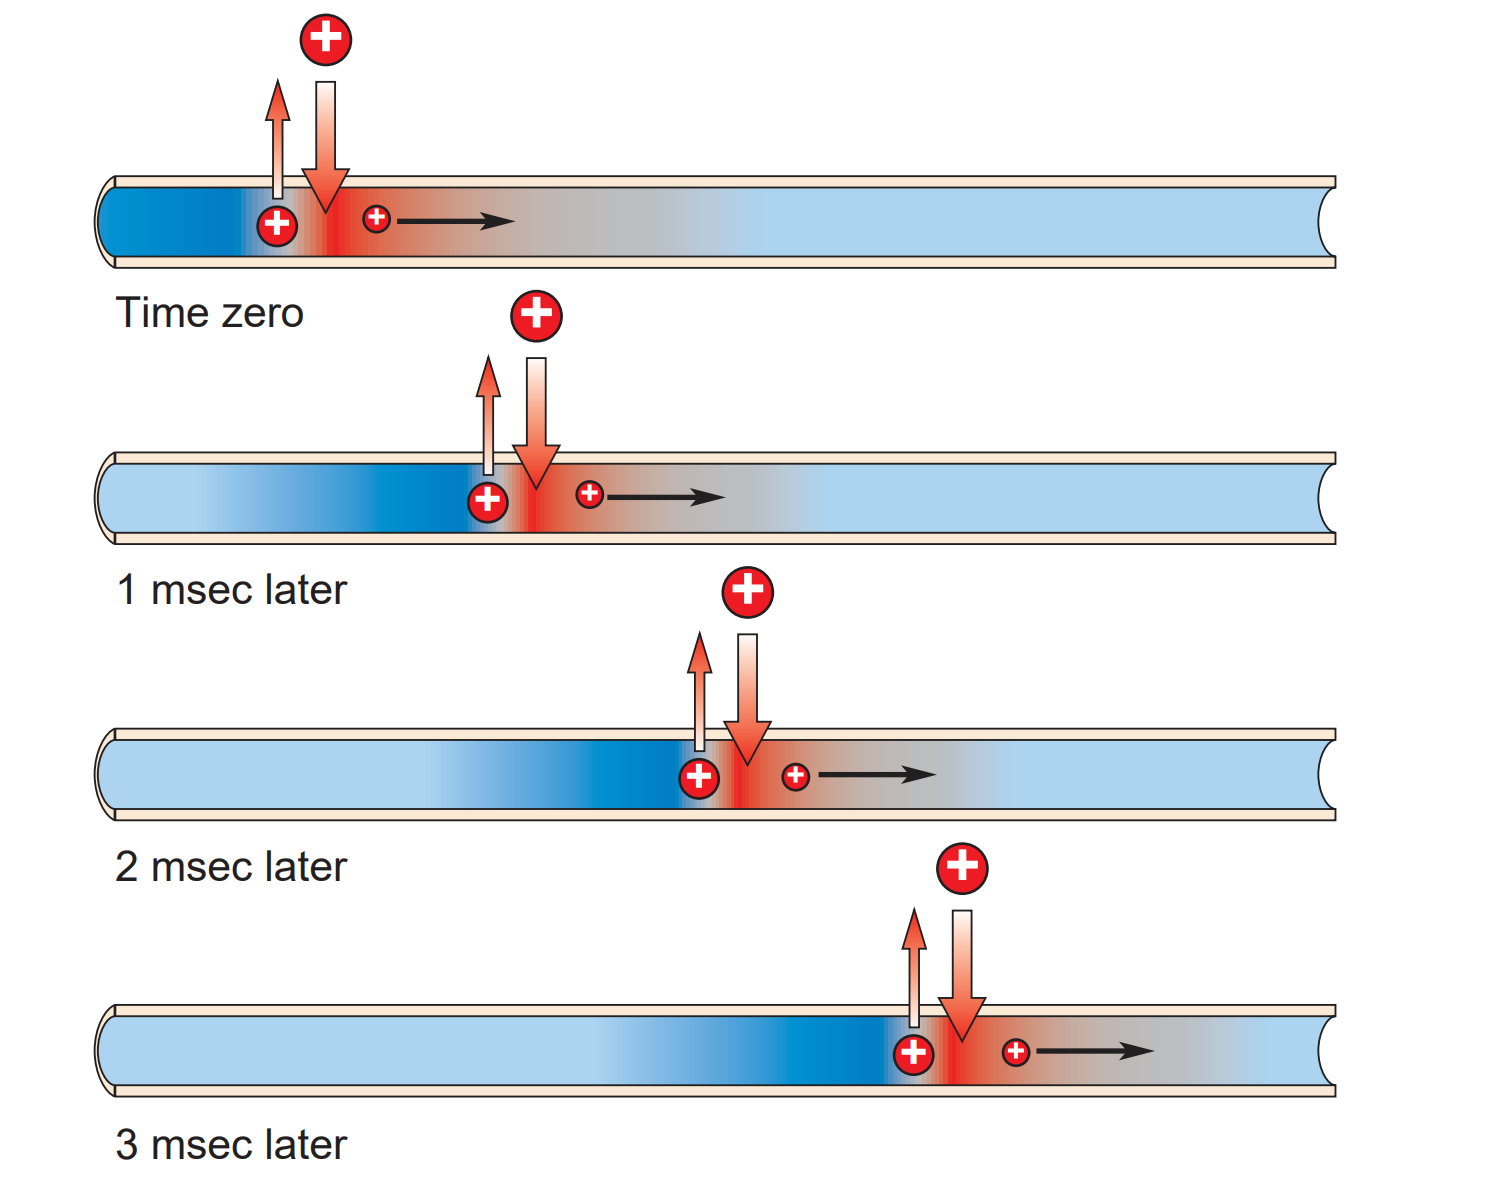
\includegraphics[width=0.4\linewidth]{Pictures/Svet/Screenshot (903).png}
  \caption{\textbf{Signal propagation in the axon segment.} The action potential's positive charge influx prompts the membrane in front to depolarize by reaching the threshold.}\label{fig:cond}
\end{figure}

\subsubsection{Unitary currents}
The \unit[per-mode = symbol]{\ucur\sodium\per\V} relation is obtained by plotting the amplitude of the unitary current \(\br{\ucur\sodium}\) versus \gls{gls:mPote} \(\br{\unit{\V\membrane}}\). This relation is linear between \qtyrange{-50}{0}{\mV}. For \glspl{gls:mPote} \gls{gls:hypol} beyond \qty{-50}{\mV}, \(\ucur\sodium\) will have close to no value. As illustrated by \cref{eq:Na}, the \gls{Na} channel has a reduced strength of gradient, drastically lowering the probability of opening \cite{Hammond2015ch4}.
\footnote{Quantitative data for \glspl{gls:mPote} more depolarized than \qty{0}{\mV} is, \emph{bizarrely}, lacking.}
 
The critical point of the current/voltage relation is the \gls{gls:mPote} for which the current is zero; i.e. the \gls{gls:rPote} of the current \(\br{\equi\reverse}\). 
Because exclusively \gls{Na} \glspl{gls:ion} flow through \gls{Na} channels, the \gls{gls:rPote} is equal to \(\equi\sodium\). 
From \qty{-50}{\mV} to \(\equi\reverse\), \(\ucur\sodium\) is inward and its amplitude decreases. This results from the decrease of the \gls{Na} driving potential \(\br{\unit{\V\membrane}-\equi\sodium}\) as the \gls{gls:membrane} approaches the \gls{gls:rPote} for \gls{Na} \glspl{gls:ion}. 
For \glspl{gls:membrane} \gls{gls:depol} greater than \(\equi\reverse\), \(\ucur\sodium\) is now outward. Above \(\equi\reverse\), the amplitude of the outward \gls{Na} current progressively increases as the driving potential for the exit of \gls{Na} \glspl{gls:ion} increases. 

The relation \unit[per-mode = symbol]{\ucur\sodium\per\V} is \gls{gls:linear}[ly] described by the equation \(\ucur\sodium = \ucon\sodium \br{\unit{\V\membrane}-\equi\sodium}\), where \unit{\V\membrane} is the test potential, \(\equi\sodium\) is the \gls{gls:rPote} of the \gls{Na} current, and \(\ucon\sodium\) is the \gls{gls:admit} of a single \gls{Na} channel (unitary \gls{gls:admit}). The value of \(\ucon\sodium\) is given by the slope of the linear \unit[per-mode = symbol]{\ucur\sodium\per\V} curve. It has a constant value at any given \gls{gls:mPote}. This value varies between \qtyrange{5}{18}{\pico\siemens} depending on the preparation.

The probability of \gls{gls:vgate}[d] \gls{Na} channels opening is dependent on voltage and time. 
During cell recordings of \gls{Na} channels, observations showing that when the \gls{gls:mPote} depolarizes, the probability of the \gls{Na} channel being in the open state increases proportional to \gls{gls:depol} until reaching a maximal level~\cite{Hammond2015ch4}. 
The greater the \gls{gls:depol}, the higher is the probability of an individual \gls{Na} channel opening. 
Variation also comes from the time, with greater probability of a channel opening towards the start of \gls{gls:depol}.
Additional observations show that after \qtyrange{4}{6}{\ms}, the probability of the \gls{Na} channel being in the open state decreases drastically~\cite{Hammond2015ch4}. 
Even with a large \gls{gls:depol} step: the \gls{Na} channel inactivates after \qtyrange{4}{6}{\ms}~\cite{Hammond2015ch4}. 

{}\(\curr\sodium\) is the macroscopic current, or the sum of all unitary currents \(\ucur\sodium\) flowing through all the open \gls{Na} channels of the \gls{gls:membrane} being recorded. Shown in \Cref{fig:unitcurNa}b, an average of \(\num{300}\) unitary \gls{Na} currents elicited by a \gls{gls:depol} pulse of \(\qty{40}{\mV}\). 
For any given potential, the average of inward \gls{gls:flux} for \gls{Na} rises quickly, reaching the peak at time, \(t=\qty{1.5}{\ms}\) \cite{Hammond2015ch4}. 
The peak corresponds to the time when most of the \gls{Na} channels are opened at each trial. 
Subsequently, the average now decays with time because the \gls{Na} channels have a proportionately lower probability of being open.\footnotemark~At each trial, the \gls{Na} channel does not trigger inactivation at exactly the same time, which explains the progressive decay of the average macroscopic \gls{Na} current. 
\footnotetext{Owing to the inactivation of the \gls{Na} channel.}

\begin{figure}[H]
  \centering
  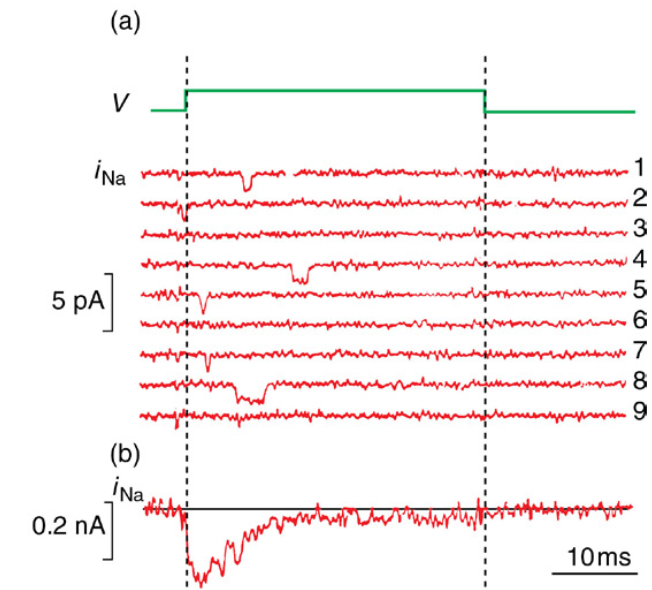
\includegraphics[width=0.5\linewidth]{Pictures//Anakin/iNa.png}
  \caption{Single \gls{Na} channel openings in response to a depolarizing step. (a) Nine successive recordings of single channel openings (\(\ucur\sodium\)) in response to a \qty{40}{\mV} depolarizing pulse (V trace in green) applied at 1s intervals from resting \gls{gls:mPote}. (b) Averaged inward \gls{Na} current from 300 elementary \gls{Na} currents as in (a). Adapted from Sigworth FJ, Neher e (1980) Single \gls{Na} channel currents observed in rat muscle cells. Nature287, 447–449 }
  \label{fig:unitcurNa}
\end{figure}

The greater the numerical quantity of \gls{Na} channels opened by \gls{gls:depol}, the smoother the current's sum total \gls{Na} will be. 
The value of \(\curr\sodium\) at each time \(t\) at a given \gls{gls:Pote} is: 
\begin{align}
    \curr\sodium = p_t \, N \, \ucur\sodium = p_t \sum^N_{n=1} \, \sbr{\ucur\sodium}_n \label{eq:nasum}\\
    \curr\potassium = N p_o \ucur\potassium = p_o \sum^N_{n=1} \, \sbr{\ucur\potassium}_n \label{eq:ksum}
\end{align}
with \(N\) as the total number of \gls{Na} channels in the \gls{gls:membrane} being recorderd and \(p_t\) is the opening probability at time \(t\). 

Subsequently, the relation of the macroscopic \gls{Na} current \(\curr\sodium\) and voltage \(\unit{\V}\) is not linear, but rather has a recognizable skewed normal distribution, illustrated in \Cref{fig:IVdist}, with a peak at around \qty{-40}{\mV}. 
\begin{figure}[H]
  \centering
  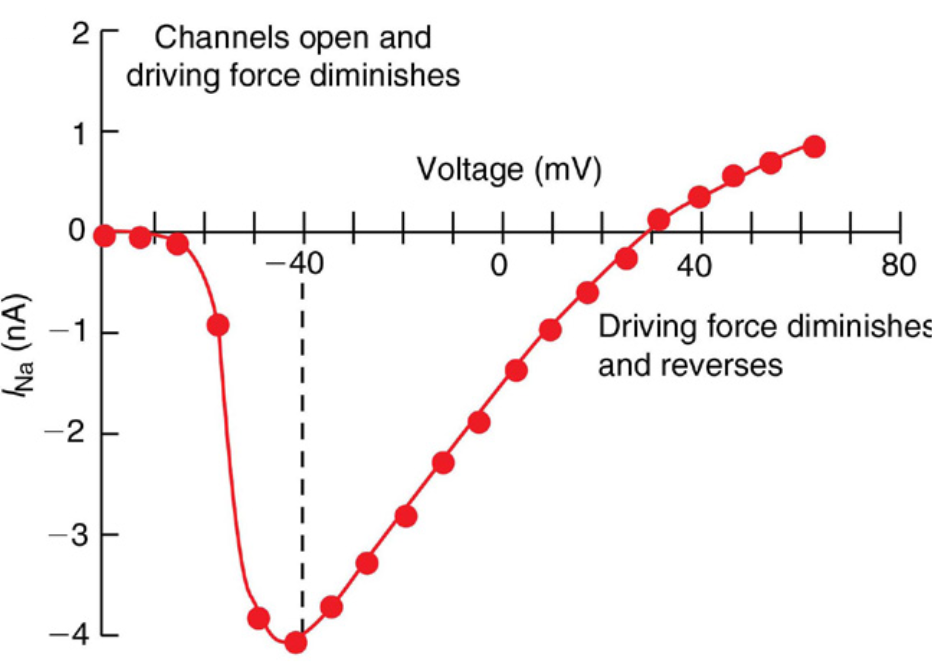
\includegraphics[width=0.5\textwidth]{Pictures//Anakin/I-V.bell.png}
  \caption{The \(\curr\sodium/\unit{\V}\) relation has a bell shape. (From Chiu Sy, ritchie JM, bogart rb, Stagg d (1979) A quantitative description of \gls{gls:membrane} currents from a rabbit myelinated nerve J. Physiol.292, 149–166)}\label{fig:IVdist.}
\end{figure}
 
For small steps, the peak amplitude of current is small, \(\br{\qty{0.2}{\nano\ampere}}\), and has a low peaking rate \(\br{\qty{1}{\milli\second}}\)~\cite{Hammond2015ch4}. At these \glspl{gls:Pote}, the \gls{Na} driving potential is strong but the \gls{Na} channels have a low probability of opening. Therefore, \(\curr\sodium\) is small since it represents the current through a small number of open \gls{Na} channels. 

As the depolarizing steps increase in amplitude \(\br{\qtyrange{-42}{-35}{\mV}}\), the amplitude of \(\curr\sodium\) increases to a maximum \(\br{\qty{-3}{\nA}}\) and the time to peak decreases to a minimum \(\br{\qty{0.2}{\ms}}\)~\cite{Hammond2015ch4}. 
Larger \glspl{gls:depol} increase probability of \gls{Na} channels being in the open state and shorten the opening delay. 
Therefore, though the amplitude of \(\ucur\sodium\) decreases by \qtyrange{-63}{-35}{\mV}, the amplitude of \(\curr\sodium\) increases, as a consequence of the increasing quantity of open \gls{Na} channels. 

After the peak, the amplitude of \(\curr\sodium\) decreases to zero, past the peak the probability of opening is no longer enough to compensate for the decrease of \(\ucur\sodium\). 
The \gls{gls:rPote} of \(\curr\sodium\) is the same as that of \(\ucur\sodium\), depending only on the \gls{gls:excell} and \gls{gls:incell} concentrations of \gls{Na} \glspl{gls:ion}.

\(\curr\sodium\) changes polarity for \unit{\V\membrane} more depolarized than Erev: it is now an outward current whose amplitude increases with the \gls{gls:depol}.


%\subsection{Application} 
%In physiological conditions, several channels of the same type are open at the same time in the \gls{gls:neuron}[al] \gls{gls:membrane}. 

%\subsubsection{Theory}

\section{The membrane as a circuit analogy}


%\subsection*{The membrane as a circuit analogy}
%The model of Hodgkin-Huxley describes the generation and propagation of an action potential in cells that are excitable. The model is based on the electrical properties of the membrane being the focal point.
%and from where the electrical circuit theory can be analogized.
The properties of the cell membrane can be compared to five electrical elements that make up a \gls{gls:circuit} and which all obey Ohm's Law. The elements are the \gls{gls:batteries}, \gls{gls:capacitor}, \gls{gls:resistor}, \gls{gls:varresistor}, and the \gls{gls:wire} is the medium in which the charges move, specifically it is the intra-/extra cellular space itself \Cref{fig:MembraneCircut}.

In the circuit diagram, the batteries also known as a \gls{gls:vsource}[s], abbreviated with the letters $E_{Na}$, $E_K$, or $E_L$ are symbolized by two parallel lines where one is longer than the other. The shorter end is the negative side (anode) and the longer end is the positive side (cathode). The function of the \gls{gls:voltage} source, in this scenario, is to facilitate the transport of charges between intra/extra-cellular space. From the perspective of the cell membrane the voltage source symbolizes ion pumps (the process is fueled by the chemical compound ATP) cf. \cref{sec:diffuseIon}. From \Cref{fig:MembraneCircut} it can be seen that there are three voltage sources two of which have the same orientation. The voltage sources \cref{tab:voltagesources} can be described as follows:

\begin{figure}[H]
    \centering
    \import{../../Pictures/Anakin}{LipidCircuit.tex}
    \caption{The Hodgkin-Huxely circuit diagram overlaid with the relevant structures found in the \gls{gls:membrane}. \glssymbol{gls:excell} and \glssymbol{gls:incell} denote the \gls{gls:excell} space and the \gls{gls:incell} space respectively. \Gls{gls:capa} of the \gls{gls:membrane} \(\br{\capa\membrane}\) is given by the charge difference on either side of the \gls{gls:bilipid}. \Glspl{gls:ionChan} for  \gls{Na} and  \gls{K} are shown with the relevant variables, resistor type, and battery. Additional \glspl{gls:ionChan} and other leaked is represented as a lone resistor and battery outside of the \gls{gls:membrane} region. The \gls{K} \glspl{gls:ion} are shown in green,  \gls{Na} are shown in red, and  \gls{Cl} \glspl{gls:ion} in yellow; distributed in approximately relative concentrations on either side of the \gls{gls:membrane}.}\label{fig:MembraneCircut}
\end{figure}
\todo{We need more}
\begin{table}[htb]
    \centering
    \caption{Voltage sources}\label{tab:voltagesources}
    \begin{tabular}{m{0.10\textwidth} @{}
                    m{0.35\textwidth}  @{}
                    m{0.50\textwidth}} \hline
        Notation & Name & Description \\\hline
$E_{Na}$ & Sodium Nernst potential & reflects the tendency of sodium ions to move \textit{into} the cell when sodium channels open \\
$E_K$ & Potassium Nernst potential & reflects the tendency of potassium ions to move \textit{out} of the cell when potassium channels open \\
$E_{L}$ & Leak channel potential & represents the electrochemical equilibrium for the leak channels, which are permeable to multiple ions. The leak current is typically more permeable to potassium at rest, so $E_L$ is closer to the potassium Nernst potential \\ \hline
\end{tabular}
\end{table}

%\begin{enumerate}
 %   \item $E_{Na}$: The Sodium Nernst Potential reflects the tendency of sodium ions to move \textit{into} the cell when sodium channels open.
%    \item $E_K$: The Potassium Nernst Potential reflects the tendency of potassium ions to move \textit{out} of the cell when potassium channels open.
 %   \item $E_{L}$: The Leak Channel Potential represents the electrochemical equilibrium for the leak channels, which are permeable to multiple ions. The leak current is typically more permeable to potassium at rest, so $E_L$ is closer to the potassium Nernst potential.
%\end{enumerate}

The circuit model of HH also contains three resistors \cref{tab:rezistors}\todo{Table not showing, so cref not working} which represent ion channels, symbolized by zig-zag lines. Two of these are voltage-dependent variable resistors (with an arrow). Their characteristics are as follows:\todo{Table: We need more of a description. Table not showing }

\begin{table}[htb]
    \centering
    \caption{Resistors}\label{tab:rezistors}
    \begin{tabular}{m{0.10\textwidth} @{}
                    m{0.35\textwidth}  @{}
                    m{0.50\textwidth}} \hline
        Notation & Name & Description \\\hline
$R_{Na}$ & Sodium Channels & allow sodium ions to flow into the cell when open, contributing to depolarization \\
$R_K$ & Potassium Channels & allow potassium ions to flow out of the cell when open, contributing to re-polarization \\
$R_{leak}$ & Leak Channels & non-specific leak channels that allow a small constant flow of ions across the membrane, contributing to the resting membrane potential \\ \hline
\end{tabular}
\end{table}


The last component or structure is that of the membrane symbolized by a capacitor. It effectively stores electrical charge and influences the rate by which the membrane change potential.
The external stimuli is symbolized by the letter $I$ and is the flow of charge particles released from the opening of ion channels. It represents any influence or perturbation that can alter the membrane potential of the neuron and potentially lead to the generation of an action potential, e.g. synaptic input, sensory stimulation, hormonal Influence \cite{EEGbook}.

The arrangement of these components in the circuit diagram is not random but rather reflects the spatial and functional organization of ion channels, their associated ion gradients, and the electrical capacitance of the membrane \cite{Shadizadeh2022}.

The ionic electrical current \(\curr\ion\), is a net transition of a specific ion through the cellular membrane \cite{wood1996neuroscience}. It flows in both types of voltage-gated channels and can be computed using an adapted form of Ohm's law \cite{kandel2000principles}. It is a simplistic model, which was proposed by Hodgkin and Huxley. It incorporates both electrical (\unit{\V\membrane}) and chemical ionic driving forces (\(\equi\sodium\), \(\equi\potassium\)) on sodium and potassium ions \cite{kandel2000principles}. The magnitude of a particular ionic current \(\curr\ion\), is given by:

\begin{align}
    \curr\sodium &= \unit{\cond\sodium} \, \br{\unit{\V\membrane} - \equi\sodium}\label{eq:sodiumCurrent}\\
    \curr\potassium &= \unit{\cond\potassium} \, \br{\unit{\V\membrane} - \equi\potassium}\label{eq:potassiumCurrent}
\end{align}

where \unit{\cond\sodium} and \unit{\cond\potassium} are ionic conductances, indicating the number of currently active channels, and (\unit{\V\membrane} - \(\curr\ion\)) is the ionic electrochemical driving force between the membrane and equilibrium potential, respectively. For as long as there is a disparity between \(\curr\ion\) and \unit{\V\membrane}, the current will be flowing \cite{wood1996neuroscience}. 


The membrane potential \unit{\V\membrane}, is an independent variable defined by a researcher. The ionic currents \unit{\curr\sodium}, \unit{\curr\potassium} on the other hand, are dependent variables whose values may be obtained from the voltage-clump test \cite{kandel2000principles}. Equilibrium potentials \(\equi\sodium\), \(\equi\potassium\) are parameters, which values can be measured experimentally 
\cite{kandel2000principles}\footnote{Look for the value of the membrane potential where ionic currents \unit{\curr\sodium}, \unit{\curr\potassium} switch the polarity; i.e., reversal potentials \(\equi\reverse\) \cite{kandel2000principles}.}.
Lastly, the ionic conductances \unit{\cond\sodium}, \unit{\cond\potassium} may be computed numerically, by re-arranging \Cref{eq:potassiumCurrent,eq:sodiumCurrent}. 



Preceding formulas \Cref{eq:potassiumCurrent,eq:sodiumCurrent} can be deduced from the analysis of an analogous circuitry. Recall that (voltage-gated) conductive channels with conductances \unit{\cond\sodium}, \unit{\cond\potassium} are, due to their time- and voltage-dependency, dependent variables. They are pictured as conductors (resistors) with an arrow across; a sign for variable conductances. They are aligned in series with batteries $E_{Na}$, $E_{K}$, that are symbolizing chemical gradients (driving forces) for sodium and potassium ions. Together, batteries and conductances, account for the voltage-dependent ionic currents \unit{\curr\sodium}, \unit{\curr\potassium}: an early transient inward \gls{Na} current which depolarizes the \gls{gls:membrane}, and a delayed outward \gls{K} current largely responsible for \gls{gls:repol} \cite{HodHux1952} \cite{kandel2000principles}.

Leakage channels, on the contrary, are commonly treated as constants or parameters in modelling. At rest, these (passive) channels are open, permitting ions to undergo passive diffusion across the cell membrane. They are represented as conductances ($g_{leak}$) with fixed values, which remain unaffected by any voltage alterations (no arrow). Leakage conductances play a pivotal role as mechanism allowing neurons to regulate their resting membrane potentials \unit{\V\membrane}. The leakage conductance $g_{leak}$ in series with its corresponding battery $E_{leak}$, account for the leakage current $I_{leak}$ \cite{kandel2000principles}. 

Whereas the movement of ions, like sodium and potassium, constitutes ionic currents across the membrane, cellular membrane exhibits a capacitive behaviour which originates from its lipid bilayer, reflecting the membrane's ability to store and discharge an electrical charge on its surfaces and react to voltage shifts. Ultimately, the membrane capacitance $C_{m}$ is connected in parallel with voltage-gated conductive passageways, remaining indifferent to ionic currents, which symbolizes its independent functioning. Please note the direction of the ionic current flow, is a response to depolarization process \cite{kandel2000principles}.


% \section{Voltage and Current}
% The flow of charge is called current. Current is measured by the number of charges that pass through a boundary per unit of time. The symbol for current is I and its unit is Ampere. The formula for current is derived from Ohm's law. Ohm's law is \(V=IR\), where \glssymbol{gls:volt} is the voltage, \(I\) is the current, and \(R\) is the resistance. Voltage is synonymous with electric pressure. This pressure pushes the current through a loop in order for it to produce some kind of work \cite{}. 


\end{document}